
% \begin{table}
% 	\centering
% 	\begin{tabular}{c|c|c|}
% 		& \textbf{Singular/Total} & \textbf{Per Node}
% 		\\ \hline
% 		Value stored & \(N^3\) & \(\frac{N^3}{\#P}\) 
% 	\end{tabular}
% 	\caption{Assuming that the grid is threedimensional and has \(N_x=N_y=N_z=N\) grid points in each direction. Contents of the grid structures as a total, and divided on each computational node.}
% \end{table}

\tikzstyle{vertex}=[circle,fill=black!25,minimum size=20pt,inner sep=0pt]
\tikzstyle{ghost}=[circle,fill=blue!25,minimum size=20pt,inner sep=0pt]
\tikzstyle{overlap}=[circle,fill=red!50,minimum size=20pt,inner sep=0pt]

	

	%Note to self: This should really have been done in a more automated/smarter way
	\begin{figure}
		\centering
		\begin{subfigure}[b]{1\textwidth}
		\centering
		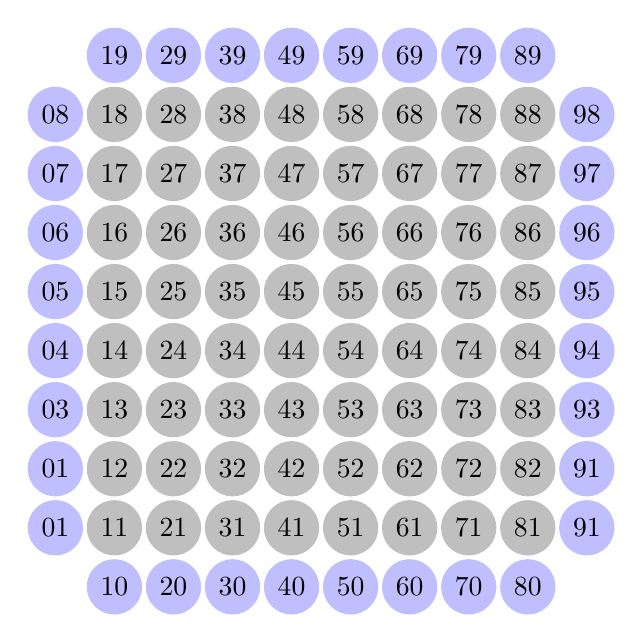
\begin{tikzpicture}[scale=0.75, auto,swap]
	    	%Adding the ghost nodes along the edges
	    	\foreach \pos/\name in 	{				{(1,0)/10}, 	{(2,0)/20},		{(3,0)/30},
	    							 {(4,0)/40},	{(5,0)/50}, 	{(6,0)/60},		{(7,0)/70},
	    							 {(8,0)/80}}
		    \node[ghost] (\name) at \pos {$\name$};
		    \foreach \pos/\name in 	{{(0,1)/01}, 	{(0,2)/01},		{(0,3)/03},
									{(0,4)/04},		{(0,5)/05}, 	{(0,6)/06},		{(0,7)/07},
									{(0,8)/08}}
		    \node[ghost] (\name) at \pos {$\name$};
		    \foreach \pos/\name in 	{	{(1,9)/19}, 	{(2,9)/29},		{(3,9)/39},
	    							 {(4,9)/49},	{(5,9)/59}, 	{(6,9)/69},		{(7,9)/79},
	    							 {(8,9)/89}}
		    \node[ghost] (\name) at \pos {$\name$};
		    \foreach \pos/\name in 	{	{(9,1)/91}, 	{(9,2)/91},		{(9,3)/93},
									{(9,4)/94},		{(9,5)/95}, 	{(9,6)/96},		{(9,7)/97},
									{(9,8)/98}}
		    \node[ghost] (\name) at \pos {$\name$};
		    %The inner nodes
		    \foreach \pos/\name in {{(1,1)/11}, 	{(1,2)/12},		{(1,3)/13},		{(1,4)/14},
		    						{(1,5)/15}, 	{(1,6)/16},		{(1,7)/17},		{(1,8)/18}}
		    \node[vertex] (\name) at \pos {$\name$};
		    \foreach \pos/\name in {{(2,1)/21}, 	{(2,2)/22},		{(2,3)/23},		{(2,4)/24},
		    						{(2,5)/25}, 	{(2,6)/26},		{(2,7)/27},		{(2,8)/28}}
		    \node[vertex] (\name) at \pos {$\name$};
		    \foreach \pos/\name in {{(3,1)/31}, 	{(3,2)/32},		{(3,3)/33},		{(3,4)/34},
		    						{(3,5)/35}, 	{(3,6)/36},		{(3,7)/37},		{(3,8)/38}}
		    \node[vertex] (\name) at \pos {$\name$};
		    \foreach \pos/\name in {{(4,1)/41}, 	{(4,2)/42},		{(4,3)/43},		{(4,4)/44},
		    						{(4,5)/45}, 	{(4,6)/46},		{(4,7)/47},		{(4,8)/48}}
		    \node[vertex] (\name) at \pos {$\name$};
		    \foreach \pos/\name in {{(5,1)/51}, 	{(5,2)/52},		{(5,3)/53},		{(5,4)/54},
		    						{(5,5)/55}, 	{(5,6)/56},		{(5,7)/57},		{(5,8)/58}}
		    \node[vertex] (\name) at \pos {$\name$};
		    \foreach \pos/\name in {{(6,1)/61}, 	{(6,2)/62},		{(6,3)/63},		{(6,4)/64},
		    						{(6,5)/65}, 	{(6,6)/66},		{(6,7)/67},		{(6,8)/68}}
		    \node[vertex] (\name) at \pos {$\name$};
		    \foreach \pos/\name in 	{{(7,1)/71}, 	{(7,2)/72},		{(7,3)/73},		{(7,4)/74},
		    						{(7,5)/75}, 	{(7,6)/76},		{(7,7)/77},		{(7,8)/78}}
		    \node[vertex] (\name) at \pos {$\name$};
		    \foreach \pos/\name in 	{{(8,1)/81}, 	{(8,2)/82},		{(8,3)/83},		{(8,4)/84},
		    						{(8,5)/85}, 	{(8,6)/86},		{(8,7)/87},		{(8,8)/88}}
		    \node[vertex] (\name) at \pos {$\name$};
	    \end{tikzpicture}
	    \caption{The grid points needed for an \(8\cross8\) domain.}
		\end{subfigure}
		\begin{subfigure}[b]{1\textwidth}
		\centering
		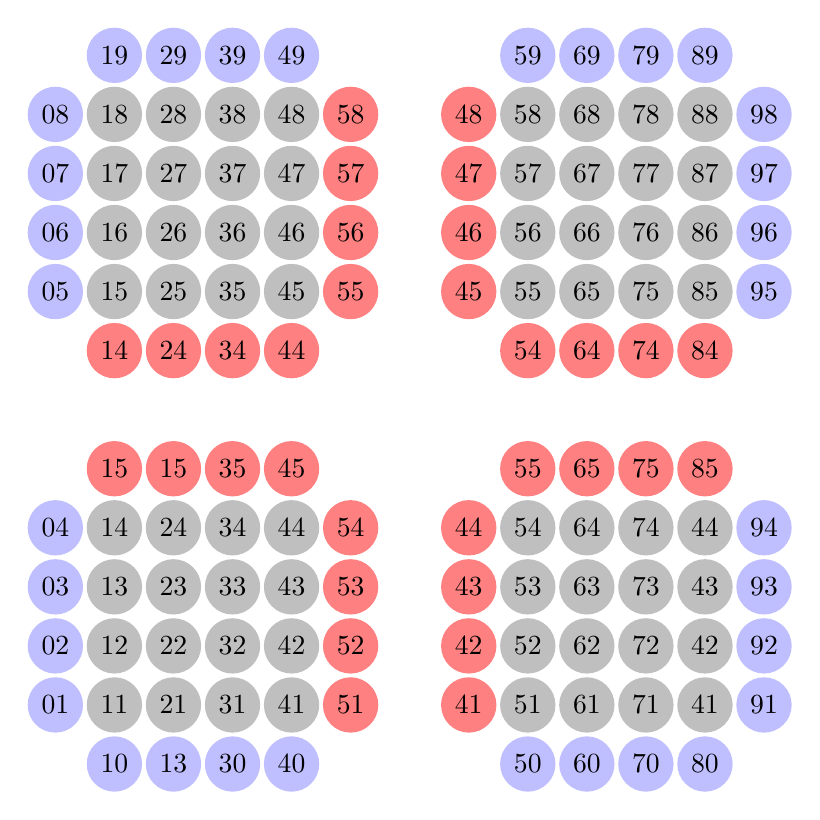
\begin{tikzpicture}[scale=0.75, auto,swap]
	    	%Left bottom corner inner
	    	\foreach \pos/\name in 	{{(1,1)/11}, 	{(1,2)/12},		{(1,3)/13},		{(1,4)/14},
		    						{(2,1)/21}, 	{(2,2)/22},		{(2,3)/23},		{(2,4)/24},
		    						{(3,1)/31}, 	{(3,2)/32},		{(3,3)/33},		{(3,4)/34},
		    						{(4,1)/41}, 	{(4,2)/42},		{(4,3)/43},		{(4,4)/44}}
		    \node[vertex] (\name) at \pos {$\name$};
		    %Left bottom corner outer
		    \foreach \pos/\name in 	%Bottom
		    	{{(1,0)/10},		{(2,0)/13},		{(3,0)/30},		{(4,0)/40}}
		    \node[ghost] (\name) at \pos {$\name$};
		    \foreach \pos/\name in 	%Top
		    	{{(1,5)/15},		{(2,5)/15},		{(3,5)/35},		{(4,5)/45}}
		    \node[overlap] (\name) at \pos {$\name$};
		    \foreach \pos/\name in 	%Left
		    	{{(0,1)/01}, 	{(0,2)/02},		{(0,3)/03},		{(0,4)/04}}
		    \node[ghost] (\name) at \pos {$\name$};
		    \foreach \pos/\name in 	%Right
		    	{{(5,1)/51}, 	{(5,2)/52},		{(5,3)/53},		{(5,4)/54}}
		    \node[overlap] (\name) at \pos {$\name$};
		    %Left bottom corner inner
	    	\foreach \pos/\name in 	{{(8,1)/51}, 	{(8,2)/52},		{(8,3)/53},		{(8,4)/54},
		    						{(9,1)/61}, 	{(9,2)/62},		{(9,3)/63},		{(9,4)/64},
		    						{(10,1)/71}, 	{(10,2)/72},	{(10,3)/73},	{(10,4)/74},
		    						{(11,1)/41}, 	{(11,2)/42},	{(11,3)/43},	{(11,4)/44}}
		    \node[vertex] (\name) at \pos {$\name$};
		    %Right bottom corner outer
		    \foreach \pos/\name in 	%Bottom
		    	{{(8,0)/50},		{(9,0)/60},		{(10,0)/70},		{(11,0)/80}}
		    \node[ghost] (\name) at \pos {$\name$};
		    \foreach \pos/\name in 	%Top
		    	{{(8,5)/55},		{(9,5)/65},		{(10,5)/75},		{(11,5)/85}}
		    \node[overlap] (\name) at \pos {$\name$};
		    \foreach \pos/\name in 	%Left
		    	{{(7,1)/41}, 	{(7,2)/42},		{(7,3)/43},		{(7,4)/44}}
		    \node[overlap] (\name) at \pos {$\name$};
		    \foreach \pos/\name in 	%Right
		    	{{(12,1)/91}, 	{(12,2)/92},	{(12,3)/93},		{(12,4)/94}}
		    \node[ghost] (\name) at \pos {$\name$};
		    %Left top corner inner
	    	\foreach \pos/\name in 	{{(1,8)/15}, 	{(1,9)/16},		{(1,10)/17},		{(1,11)/18},
		    						{(2,8)/25}, 	{(2,9)/26},		{(2,10)/27},		{(2,11)/28},
		    						{(3,8)/35}, 	{(3,9)/36},		{(3,10)/37},		{(3,11)/38},
		    						{(4,8)/45}, 	{(4,9)/46},		{(4,10)/47},		{(4,11)/48}}
		    \node[vertex] (\name) at \pos {$\name$};
		    %Left top corner outer
		    \foreach \pos/\name in 	%Bottom
		    	{{(0,8)/05},	{(0,9)/06},		{(0,10)/07},	{(0,11)/08}}
		    \node[ghost] (\name) at \pos {$\name$};
		    \foreach \pos/\name in 	%Top
		    	{{(5,8)/55},	{(5,9)/56},		{(5,10)/57},	{(5,11)/58}}
		    \node[overlap] (\name) at \pos {$\name$};
		     \foreach \pos/\name in %Left
		    	{{(1,7)/14}, 	{(2,7)/24},		{(3,7)/34},		{(4,7)/44}}
		    \node[overlap] (\name) at \pos {$\name$};
		    \foreach \pos/\name in 	%Right
		    	{{(1,12)/19}, 	{(2,12)/29},	{(3,12)/39},	{(4,12)/49}}
		    \node[ghost] (\name) at \pos {$\name$};
		    %Right top corner inner
	    	\foreach \pos/\name in 	{{(8,8)/55}, 	{(8,9)/56},		{(8,10)/57},		{(8,11)/58},
		    						{(9,8)/65}, 	{(9,9)/66},		{(9,10)/67},		{(9,11)/68},
		    						{(10,8)/75}, 	{(10,9)/76},	{(10,10)/77},		{(10,11)/78},
		    						{(11,8)/85}, 	{(11,9)/86},	{(11,10)/87},		{(11,11)/88}}
		    \node[vertex] (\name) at \pos {$\name$};
		    %Right top corner outer
		    \foreach \pos/\name in 	%Bottom
		    	{{(7,8)/45},	{(7,9)/46},		{(7,10)/47},	{(7,11)/48}}
		    \node[overlap] (\name) at \pos {$\name$};
		    \foreach \pos/\name in 	%Top
		    	{{(12,8)/95},	{(12,9)/96},	{(12,10)/97},	{(12,11)/98}}
		    \node[ghost] (\name) at \pos {$\name$};
		     \foreach \pos/\name in %Left
		    	{{(8,7)/54}, 	{(9,7)/64},		{(10,7)/74},	{(11,7)/84}}
		    \node[overlap] (\name) at \pos {$\name$};
		    \foreach \pos/\name in 	%Right
		    	{{(8,12)/59}, 	{(9,12)/69},	{(10,12)/79},	{(11,12)/89}}
		    \node[ghost] (\name) at \pos {$\name$};
	    \end{tikzpicture}
	    \caption{The \(8\cross8\) grid diveded into 4 subdomains}
		\end{subfigure}
		\caption{Each circle in the figures represents 1 grid point, and the first number is the column while the second is the row. The grey colour represents physical space the computational node works on, the blue color is the outer grid points for boundary conditions and the red colour is the overlapping grid points.}
    \end{figure}

